\documentclass[a4paper,10pt]{scrbook}
\usepackage[utf8x]{inputenc}
\usepackage[german]{babel}
\usepackage[top=2cm]{geometry}
\usepackage{enumerate}
\usepackage{framed}
\usepackage{amsmath}
\usepackage{graphicx}
\usepackage{parskip}
\usepackage{fancyhdr}
%opening
\title{WST Vogt - Lösungen}
\author{Roland Hediger}

\begin{document}

\maketitle
\pagestyle{fancy}
\chapter*{Serie 1}

\section*{Aufgabe 1}
Trivial.
\section*{Aufgabe 2}
Binär auflösen mit 0 für unbrauchbar, 1 für Brauchbar.

\section*{Aufgabe 3}
\begin{enumerate}
 \item $P(E) = \frac{3}{6}$
 \item $P(E) = \frac{6}{36}$
 \item Zweimaligs Werfen einer Munze, Erreignis ``zweimal Kopf'': \\
 $ \Omega = \{Z,K\}^2 , E = \{K,K\} P(E) = \frac{1}{4}$
 \item Züfalliges Ausfüllen eines Multiple Choice Tests mit 4 Fragen a 2 Atwortmöglichkeiten, von jeweils genau eine 
richtig ist. Erreignis mindestens hälfte richtig:
$\Omega = {r,f}^4 E=$ Tuppel mit Anzahl r höher als 1/2. $P(E) = \frac{11}{16}$
\end{enumerate}

\section*{Aufgabe 4}
In folgender Situation a) jeder, b) niemand bekommt sein eigenes Geschenk an Weinachtsparty. 3 Leute sind teilnehmer.
Es bezeichne $(a_1,a_2,a_3)$ den Fall das Person i Geschenk $a_i$ bekommt : \\
$\{(1,2,3)(3,2,1)(2,1,3)...\}$
a) $P(E) = 1/6$
b) $P(E) = 1/3 = 3/6$

\section*{Aufgabe 5} 
2*1/6 nicht gleich 11/36

\section*{Aufgabe 6}
Pin 0..9 Wie lang muss pin sein damit erraten höchstens 1\% ist. \\
$|E| = 1 P(E) ) 1/10^n \leq 0.01 n \ge 2$
\section*{Aufgabe 7}
Länge 4 Ziffern pw, 1)erste Zahl kein 0, 2) kein 0, mindestens 1 0, 1 höchstens so gross wie die anderen zahlen sein 
darf

\begin{enumerate}
 \item 1 9.10.10.10
 \item 9.9.9.9
 \item $10^4-9^4$ max - die mit kein 0
 \item $M_i$ erfüllt bedingung $1^3 + 2^3 + + 10^3 = 55^3$
\end{enumerate}

\section*{Aufgabe 8} Trivial.
\section*{Aufgabe 9} Nur 3 personen haben Führerschein. 3 für Fahrer. Dann 4 Leute übrig,dann 3 2 1 = 3.4.3.2.1
\section*{Aufgabe 10} Dualzahlen beginnen mit 11 oder enden mit 00. Funfstellig.\\
3 dynamische positionen. 2^3+2^3 - eine der 1100 ist.
\section*{Aufgabe 11} 9.10.10.10 = 9000.
\section*{Aufgabe 12} Variablennamen die aus mindestens drei and höchtens 5 Kleinbuctaben bestehen
$26^3+26^4+26^5$ 
\section*{Aufgabe 13} $\{0,1\}^n \rightarrow \{0,1\}$ Logikfunktionen festes n : 0,1 für jede funktion. Alle 
Binärzahlen ist $2^n$ : $2^{2^n}$ Unvollständig = $3^{2^n}$
\section*{Aufgabe 16} 1,2,7,8.9 5 möglichkeiten 5! max 1/5! = 1/1202
\section*{Aufgabe 17} 12.11.10 trivial
\section*{Aufgabe 18} $n!/(n-k)! = 8!/4! = 1680  {8 \choose 4} = 70$
\section*{Aufgabe 19} 1)5! 2) 4! selbstverständlich.
\section*{Aufgabe 20} 
\chapter*{Serie 5}
\section*{Aufgabe 1}
1) $P(0\leq X \leq 1) = \int_0^1 f(x)dx = F(1)-F(0)\\
f(x) = ax\\
F(x) = a \frac{x^2}{2} \\
\int = 0.5a - 0\\
0.5a -0 = 1 \\
0.5a = 1\\$ $\langle$ Gesamtfläche also $ lim \rightarrow \inf$ muss 1 sein.$\rangle$ \\
$0.5 * 2 = 1\\
a = 2$\\

2) Verteilungsfunktion zu F : \\
$F(x) = \int f(x) = \int (2x) dx = 2(x^2/2) = x^2 $\\
Warum 0 $ x \le 0$  oder 1.\\
3) \begin{enumerate}[a)]
    \item $P(\frac{1}{3} \le X \le \frac{3}{4}) = (3/4)^2 - (1/3)^2 = 65/144 = 0.451$
    \item $P(X \le 1/2) = F(1/2) - F(0) = 0.25\\$
    \item $P(3/4 \le X) = 9/16$ \\ 
   \end{enumerate}

   \section*{Aufgabe 2}
   $f(x) =$ $2x$ oder 0 sonnst \\
   $ F(x) = \frac{2x^3}{3}$ \\
   $E(x) = \frac{2}{3} \int x^3 = \frac{2}{3}*1$
     
\section*{Aufgabe 3}
\begin{verbatim}
  normcdf(x,0,1) 
 1. normcdf(1,0,1)
 2. 1-(normcdf(0.5,0,1)-normcdf(-0.5,0,1))
 3. normcdf(1,0,1)-normcdf(-3,0,1)
\end{verbatim}

\section*{Aufgabe 4}
\begin{verbatim}
 1.normcdf(8,2,2)-normcdf(-4,2,2)
 1.normcdf(2,1,3)
 1.normcdf(1,-1,4)-normcdf(-1,-1,4)
\end{verbatim}

   
\section*{Aufgabe 5}
Erwartung : Innherhalb Qualitätsbereich : 
$E(x) = \mu$ \\
Qualitätsbereich ist absolutwert. Deshalb liegt $\mu$ in der mitte (=0) \\
\begin{framed}
 \begin{equation}
  F(x) = P(X \leq X) \\
  P(a \leq X \leq B) = F(b) - F(a)
 \end{equation}
 
\end{framed}

Daraus folgt $P(-3.45 \leq X \leq 3.45) = $ \texttt{normcdf(3.45,0,3)-normcdf(-3.45,0,3)}

Anzahl Stucke mit gewunchten Qualität = \texttt{ans * 24} wo 24 die Ausführungen des Experiments sind.

\section*{Aufgabe 6}
\begin{enumerate}
 \item \texttt{normcdf(2.15,2.1,0.2)*100}
 \item \texttt{(normcdf(2.3,2.1,0.2)-normcdf(1.9,2.1,0.2))*100}
\end{enumerate}
\section*{Aufgabe 7}

Wahrscheinlichkeit das 1 Person $\ge$ 130 hat :
\texttt{1-normcdf(130,100,15) = 022750 }
\begin{verbatim}
 1. binocdf(2,5,0.022750) für genau 2 personen
 2. binopdf(2,5,person)+binopdf(3,5,022750)+binopdf(4,5,022750)+binopdf(5,5,022750)
\end{verbatim}
\section*{Aufgabe 8}
\begin{enumerate}
\item Logischerweise soll dass \texttt{1-normcdf(4.98,5,0.02)}
Aber der Antwort ist \texttt{normcdf(4.98,5,0.02)}
\item \texttt{1-normcdf(5.05,5,0.02)}
\item Absolutwert : $(P(5+0.03)-P(5-0.03))$ = \texttt{normcdf(5.03,5,0.02)-normcdf(4.97,5,0.02) = 0.86639} Antwort ist 
aber 1- gegebene Wert
\end{enumerate}

Problem - habe nicht das Wort Ausschlussteil im Aufgabe gelesen. Deshalb isr 1- gegebene Wert richtig.

\section*{Aufgabe 9}
Gewicht Grenze : Quantil : \% gegeben X $\le$ x wo x gesucht ist.
\begin{framed}
 norminv(x,$\mu,\sigma$)
\end{framed}

\texttt{norminv((1-0.1),80,10) = 92.8155}

\section*{Aufgabe 10}
\begin{framed}
 Standardisierung gemäss Folie - Bedeutzung :
 \begin{equation}
z = \frac{X-\mu}{\sigma} 
\end{equation}

Dieses wandelt den X in eine Normalverteilung um in eine X die in \textbf{Standardnormalverteilung} passt.
Sehr hilfreich wenn parameter fehlen wie hier $\mu$

Mittelwert = $\mu$
\end{framed}

$ P(z \leq 250) = 0,05$ \\
\texttt{norminv(250,$\mu$ 8}\\
Norminv der Standardnormalverteilung = \texttt{norminv(0.5) = z}
$P(0 \leq z) = 0.05$\\
$ z = \frac{X-\mu}{\sigma}$ \\
Solve for $\mu$ \\
$\mu$ = $((z \times 8) \times -1 )+ 250$ 

\section*{Aufgabe 11}
$P(X \leq 10mm)$ = 0.1736 
$1-P(X\leq 13mm) =$ 0.1446
$p(0 \leq z1) = 0.1736$\\
$z1 = norminv(0.1736)$ \\
$z1 = -0.94003$ \\
$ -0.94003 = \frac{10-\mu}{\sigma}$ \\
$ P(X \leq 13mm) = 1-0.1446 = 0.85540$ \\
$ z2 = 1.0599$ \\

Lösen mit matrix  Cramer Regel. ($\mu,\sigma,b$)\\
$\begin{pmatrix}
   -094003 & 1 & 10\\
   1.0599 & 1 & 13 \\
 \end{pmatrix}$
Wo (10,13) Lösungsvektor ist.


\section*{Aufgabe 12}
$ \mu = 8 \sigma = 3$ \\
$ P(x\leq X \leq 10) = 0.7 \\
f(10) - f(x) = 0.7 \\
f(x) = f(10) - 0.7 \\$
\texttt{f(x) = 0.047507 \\
norminv(0.047507) = -1.6695 }\\
$ z = \frac{x - \mu}{\sigma}$\\
\texttt{x = -1.6695 * 3 + 8 = 2.9915}

\section*{Aufgabe 13}
$\mu = E , \sigma = V $ für Normalverteilung.\\
\begin{enumerate}
 \item $P(55 \leq X) = 0.33$ \\
 $1-P(70 \leq X) = 0.05, P (70 \leq X) = 0.95$\\
 $z_1 = $ \texttt{norminv(0.33) = -0.43991}\\
 $z_2 =$ \texttt{norminv(0.95) = 1.6449 }
 Lösen mithilfe von Standardisierungsformel und Cramer Regel wie oben.
\end{enumerate}

\section*{Aufgabe 14}
\begin{enumerate}
 \item 1 wegen $ \lambda = 1$
 \item  $\delta = \sqrt(V(X)) = \sqrt{\frac{1}{1^2}} = 1$
 \item $P(T \leq 4) = $ \texttt{expcdf(4,1) = 0.982}
 \item $ P(2 \leq X \leq 5) = $ \texttt{expcdf(5,1/1)-expcdf(2,1/1) = 0.12860 = 0.129}
\end{enumerate}

\section*{Aufgabe 15}
$\lambda =  0.02$ \\
\begin{enumerate}
 \item $ P( X \geq 50) = 1-P(X \leq 50) $ = \texttt{1- expcdf(50,1/0.02)} = 0.3679
\item 0 + 20 = 30 +20 kein gedächnis. expcdf(20)	
\end{enumerate}

\section*{Aufgabe 16}
\begin{verbatim}
1) (0.2*(1-expcdf(2/60,1/10))) + (0.3*(1-expcdf(2/60,1/20))) + (0.5*(1-expcdf(
2/60,1/30))) Zeiteinheit in Stunden.
2)(0.2*(expcdf(1/120,1/10))) + (0.3*(expcdf(1/120,1/20))) + (0.5*(expcdf(1/120,1/30)))
 
\end{verbatim}

\chapter*{Serie 6}
\section*{Aufgabe 1}
\begin{verbatim}
 1. 0.6065 = 1 − expcdf (5, 10)
2. 0.1738 = (1 − expcdf (5, 10) ∗ (1 − expcdf (5, 20) ∗ (1 − expcdf (5, 5))
3. 0.9450 = 1 − expcdf (5, 10) ∗ expcdf (5, 20) ∗ expcdf (5, 5)
4. 0.6345 = (1 − expcdf (5, 10)) ∗ (1 − expcdf (5, 20)) ∗ expcdf (5, 5) + (1 − expcdf (5, 10)) ∗
expcdf (5, 20) ∗ (1 − expcdf (5, 5)) + expcdf (5, 10) ∗ (1 − expcdf (5, 20)) ∗ (1 − expcdf (5, 5)) +
(1 − expcdf (5, 10)) ∗ (1 − expcdf (5, 20)) ∗ (1 − expcdf (5, 5)
\end{verbatim}
\section*{Aufgabe 2}
\begin{verbatim}
 1. 0.6065 = 1 − expcdf (5, 10)
2. 0.1738 = (1 − expcdf (5, 10) ∗ (1 − expcdf (5, 20) ∗ (1 − expcdf (5, 5))
3. 0.9450 = 1 − expcdf (5, 10) ∗ expcdf (5, 20) ∗ expcdf (5, 5)
4. 0.6345 = (1 − expcdf (5, 10)) ∗ (1 − expcdf (5, 20)) ∗ expcdf (5, 5) + (1 − expcdf (5, 10)) ∗
expcdf (5, 20) ∗ (1 − expcdf (5, 5)) + expcdf (5, 10) ∗ (1 − expcdf (5, 20)) ∗ (1 − expcdf (5, 5)) +
(1 − expcdf (5, 10)) ∗ (1 − expcdf (5, 20)) ∗ (1 − expcdf (5, 5))
\end{verbatim}

\section*{Aufgabe 3}
\begin{verbatim}
1. 0.0234 = (1 − poisscdf (1, 3)) ∗ poisscdf (4, 10)
2. 0.9032 = 1 − poisscdf (19, 26)
\end{verbatim}
2. 3 im schnitt 1 Stunde , 6 im Schnitt 2 Stunden. 20 im Schnitt Mobil daraus folgt 6+20 = 26

\section*{Aufgabe 4}
\begin{figure}[h]
 \centering
 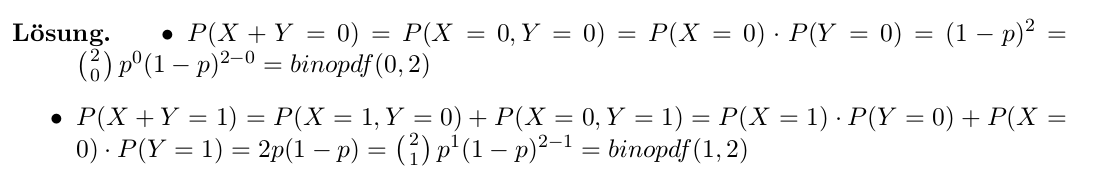
\includegraphics[scale=0.4]{./a4s6.png}
 % a4s6.png: 1107x195 pixel, 72dpi, 39.05x6.88 cm, bb=0 0 1107 195
\end{figure}

\section*{Aufgabe 5}
$ E_{wurfel} =$ E(Bin(10,1/6))  \\
$ = 10*1/6$ \\
$ E_{zahl} = $ E(Geo) $ = 1/\frac{1}{2}$ \\
$E_{gesamt} = 1*2 + 10/6 -1 $ -1 weil wir für nicht treffer suchen.


\section*{Aufgabe 6}

1) 400+4*30 $\mu_1 + \mu_2*4$
2) \begin{verbatim}
    1-normcdf(530,520,sqrt(10^2+4*5^2)
   \end{verbatim}
   Unabhängige Zufallsvariablen  Folie 7
3) a) Nicht gekater Anteil  : 
\begin{verbatim}
 0.1855 = normcdf (500, 520, sqrt(10**2 + 16 ∗ 5**2 ))// ** = hoch etwas
\end{verbatim}
3 b) Nicht verkaufte anteil = a daraus folgt gekaufter Anteil ist 1- a)
Bino Verteilung (n,1-a)) 
3c) P(X $\ge$ 100) = 90\% aber norminv funktioniert nur fur $\le$ daraus folgt  1- P(X$\ge$ 100) = 10\% = norminv(0.1)\\
$\mu $ und $\sigma$ gegeben durch a)\\
\textbf{Standardisierungsformel von oben}:
\begin{figure}[h]
 \centering
 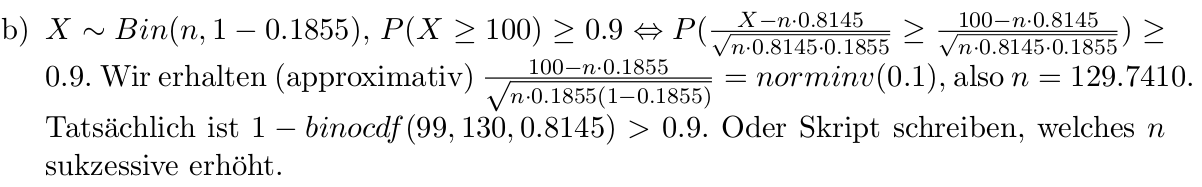
\includegraphics[scale=0.4]{./kuchen.png}
 % kuchen.png: 1202x187 pixel, 72dpi, 42.40x6.60 cm, bb=0 0 1202 187
\end{figure}
4) \begin{verbatim}
    556.78 = norminv(0.95, 520, sqrt(10**2 + 16 ∗ 5**2 ))
   \end{verbatim}
\section*{Aufgabe 7}
\begin{framed}
 Tschebbycheff oder was auch immer :
 \begin{equation}
  P(|X - \mu|) \ge k) \le \frac{\sigma^2}{k^ 2}
 \end{equation}

\end{framed}
$ P(|X-100| \ge 20) \le 0.2025$

\chapter*{Serie 7}
\section*{Aufgabe 1}
$z_a = z_\alpha$\\
2994 Kinder 1562 Knaben.
Sei $X=k$ wo $n = 2994$ dann ist $k =1562$
Sei $z_a$ das Quantil für $N(0,1)$ $z_a$ = norminv(a) $ a = \frac{1 + Q}{2}$ \\
$ a = 1.95/2 = 0.97500$ \\
norminv(97.500) = $z_a$ = 1.96\\
\begin{framed}
KonfidenzIntervall:\\
 \begin{equation}
  [\frac{k}{n} - \frac{z_a}{n} \sqrt{\frac{k(n-k)}{n}},\frac{k}{n}+\frac{z_a}{n} \sqrt{\frac{k(n-k)}{n}}]
 \end{equation}

\end{framed}

\section*{Aufgabe 2}
$z_a = z_\alpha$
$ n = 1000$\\
$ k = 30$\\
$ a = 1.9/2$ \\
norminv(a) =$ z_a$ = 1.6449
Einsetzen im Interval Formel da oben.


\section*{Aufgabe 3}
1. Ja, Additionstheorem der Normalverteilung.
2. Nein, siehe 1.
3. Ja, Additionstheorem der Normalverteilung.
4. Nein, siehe 3.

\section*{Aufgabe 4}
Verwerfungskriterium : 5 Löse aber jede Löse hat Zahl > 1600\\
$H_0$ = Es gibt 3000 Löse
1. Fehler Erste Art : 3000 Löse aber Jede von 5 < 1600 : Mehrstüfige Auswahlprozess = : \\
$\pi{n=1596}^{i=1600} \frac{l_i}{3000}$
Fehler 2 Art :\\
2000 Löse : $H_0$ trifft nicht zu aber nicht verworfen das heisst 1 minus verworfen\\
$\pi{n=1596}^{i=1600} \frac{l_i}{2000}$

3. Nicht möglich da Löse Anzahl zu wenig für Verwerfungskriterium ist. P = 0.

\section*{Aufgabe 6}
12 Karten : Anzahl Treffer - Binomial Verteilung mit p = 50\% für Treffer \\
$H_0$ = beliebig Raten
Gesucht richtige Antworten damit $H_0$ ungültig mit Signifikanznouveau  von 5\% \\

\begin{framed}
 $P(X \ge k) \le 0.05$ ist das gleiche wie $P(X \le k) \ge 0.95$ \\
 Konfidenzbereichgrenze.
\end{framed}
Invers gefragt : \\
\texttt{binoinv(0.95,12,0.5) = 9}\\
9 ist an der Grenze des ``Nicht glaubens'' daher ist es nür erfüllt bei 9+1 Karte = 10.
\end{document}